\documentclass[10pt,twocolumn,a4j]{jsarticle}
\usepackage[dvipdfmx]{graphicx}
\usepackage[subrefformat=parens]{subcaption}
\usepackage{amsmath,amssymb}
\usepackage{comment}
\setlength{\textheight}{275mm}
\headheight 5mm
\topmargin -30mm
\textwidth 185mm
\oddsidemargin -15mm
\evensidemargin -15mm
\pagestyle{empty}
\title{{\large2016年度 修士論文審査}\\非調和振動の効果を入れた有限温度の自由エネルギー計算}
\author{関西学院大学大学院理工学研究科\\情報科学専攻 西谷研究室 M5308 榊原 健}
\date{}
\begin{document}
\maketitle
\section{はじめに}
材料設計において系の有限温度における自由エネルギーの変化は基本となる物性値である.
第一原理計算は絶対零度での計算のため熱振動の効果を考慮していない.
しかしながら,熱膨張,比熱,電気伝導率などの諸物性は有限温度において振動の影響を受ける. 
そのため,有限温度での物性を計算により求めるには,
振動の効果を取り入れて計算することが必要となる.

第一原理計算ソフトVASP(Vienna ab initio simulation package) では,
擬調和振動子近似に基づいたPhonon計算パッケージが開発されており,
Phonon-DOS法を用いて自由エネルギーを見積もることができる\cite{phonon}.
しかし,Ti 結晶での相変態温度近傍での振る舞いと体積膨張率において実験を再現する結果が得られない\cite{kiyohara}.
これは相互作用の高次項である非調和項の影響が大きいためと考えられる.
%これは現実的な結晶の振る舞いを再現するためには無視することができない成分である.

Vu Van Hung らが開発したMoment 法では,
原子間の相互作用エネルギーの高次微分を考慮にいれることによって,
非調和効果を取り入れた有限温度における自由エネルギー,熱膨張などを見積もることができる\cite{jindo}.

本研究では,Moment法が前提としている経験的な原子間ポテンシャルではなく,VASPによる計算結果の組み込みを試みる.
今回は対称性に優れており等方的であるfcc金属のCu, Ag, Au, Alで計算をおこなった.
また,計算の信頼性を確かめるためにVASPを利用したPhonon-DOS法による自由エネルギーの計算ができるMedeA, Phonopyと比較した.

%本研究では,この計算手法が前提としている経験的な原子間ポテンシャルでなく,
%第一原理計算の組み込みが可能かを検証する.
%今回は,計算の妥当性を確かめるため,
%対称性の高いfcc金属のCu, Ag, Auにおいて,
%Phonon-DOS法および実験結果との比較をおこなった.

\section{Moment法}
Moment法では$i$番目の原子の平衡位置からの変位が$u_i$であり,
系に働いている外力を$a$としたときの$u_i$の平均変位を$\left<u_i\right>_a$とする.
この$\left<u_i\right>_a$を利用するのがMoment法の特徴である.
%%
\begin{comment}
$\left<u_i\right>_a$, $\left<u_i^2\right>_a$は
\begin{equation}
\left<u_i\right>_a \equiv y
\end{equation}
\begin{equation}
\left<u_i^2\right>_a = \left<u_i\right>_a^2 + \theta \frac{\delta\left<u_i\right>_a}{\delta a} + \frac{\theta}{k}(x \coth x-1)
\end{equation}
となる.ここで$\theta=k_BT$,$x=\frac{\hbar\omega}{2\theta}$, である.

$i$番目の原子とのポテンシャルを$\psi_{i0}$,平衡原子間距離を$r_0$とした場合,ポテンシャルのテイラー展開は
\begin{equation}
\begin{split}
\psi_{i0}(|r_0+u_i|)=\psi_{i0}(|r_0|)+
\frac{1}{2}\left( \frac{\delta^2\psi_{io}}{\delta u_i^2} \right) u_i^2\\+
\frac{1}{6}\left( \frac{\delta^3\psi_{io}}{\delta u_i^3} \right) u_i^3+
\frac{1}{24}\left( \frac{\delta^4\psi_{io}}{\delta u_i^4} \right) u_i^4
\end{split}
\end{equation}
と表せる.
式(1)を変位$u_i$で微分し,系全体に$a$という外力が働いている場合,
\begin{equation}
\begin{split}
\left( \frac{\delta^2\psi_{io}}{\delta u_i^2} \right) \left<u_i\right>_a+
\frac{1}{2}\left( \frac{\delta^3\psi_{io}}{\delta u_i^3} \right) \left<u_i^2\right>_a\\+
\frac{1}{6}\left( \frac{\delta^4\psi_{io}}{\delta u_i^4} \right) \left<u_i^3\right>_a- a =0
\end{split}
\end{equation}
このような等式が作れる.
ここで左辺第3項まではポテンシャルの変位微分なので変位による力を表しており,外力$a$との差が0という等式により,平衡状態を表している.この式(2)は平衡原子間距離からの変位$u$, $u^2$, $u^3$があり,$a$という外力が働いている状態なので,$\left<u_i\right>_a$,$\left<u_i^2\right>_a$,$\left<u_i^3\right>_a$を代入し原子間距離の導出に利用する.
\end{comment}
%%
\subsection{熱膨張の計算}
線形結合の系に対して$\left<u_i\right>_a$を利用することによって
外力が無い場合の変位$y_0$が得られる.
\begin{equation}
y_0= k_{\rm{B}}T\sqrt{\frac{2\gamma}{3k^3}A}
\end{equation}
$k_{\rm{B}}$はボルツマン定数,$T$は温度,$k$はポテンシャルの2次微分,$\gamma$はポテンシャルの4次微分を6で割ったもの,$A$は$k$, $\gamma$,$T$の関数であり長いため省略している.
計算者の設定する平衡原子間距離からの変位を$y$とすると,$k$, $\gamma$は$y$によって決定され,それにより$y_0$が定まる.$y_0$導出の過程で使用した式から$y$=$y_0$のとき熱膨張による平衡原子間距離からの変位が得られることがわかる.

%%
\begin{comment}
計算者が設定する平衡原子間距離からの変位を$y$,外力がない場合の平衡原子間距離からの変位を$y_0$,外力を$a$,$A_1$と$A_2$を定数とする次式を作ることができる.
\begin{equation}
y=y_0+A_1a+A_2a^2
\end{equation}
右辺第2, 3項は外力による変位を表しており,$y_0$と足し合わせることで右辺は外力の影響を考慮した変位を表している.
また,式(2),(3)から導出される$y_0$は$y$に依存する関数であり,$y$の変化に合わせて$y_0$も変化していく.
計算者が変位$y$を伸ばしていき,$y=y_0$となれば外力$a=0$となる.
このときの$y$が外力の加わっていない熱膨張のみによる原子間距離となる.
\end{comment}
%%
\begin{figure*}[htb]
\begin{minipage}{0.245\hsize}
\begin{center}
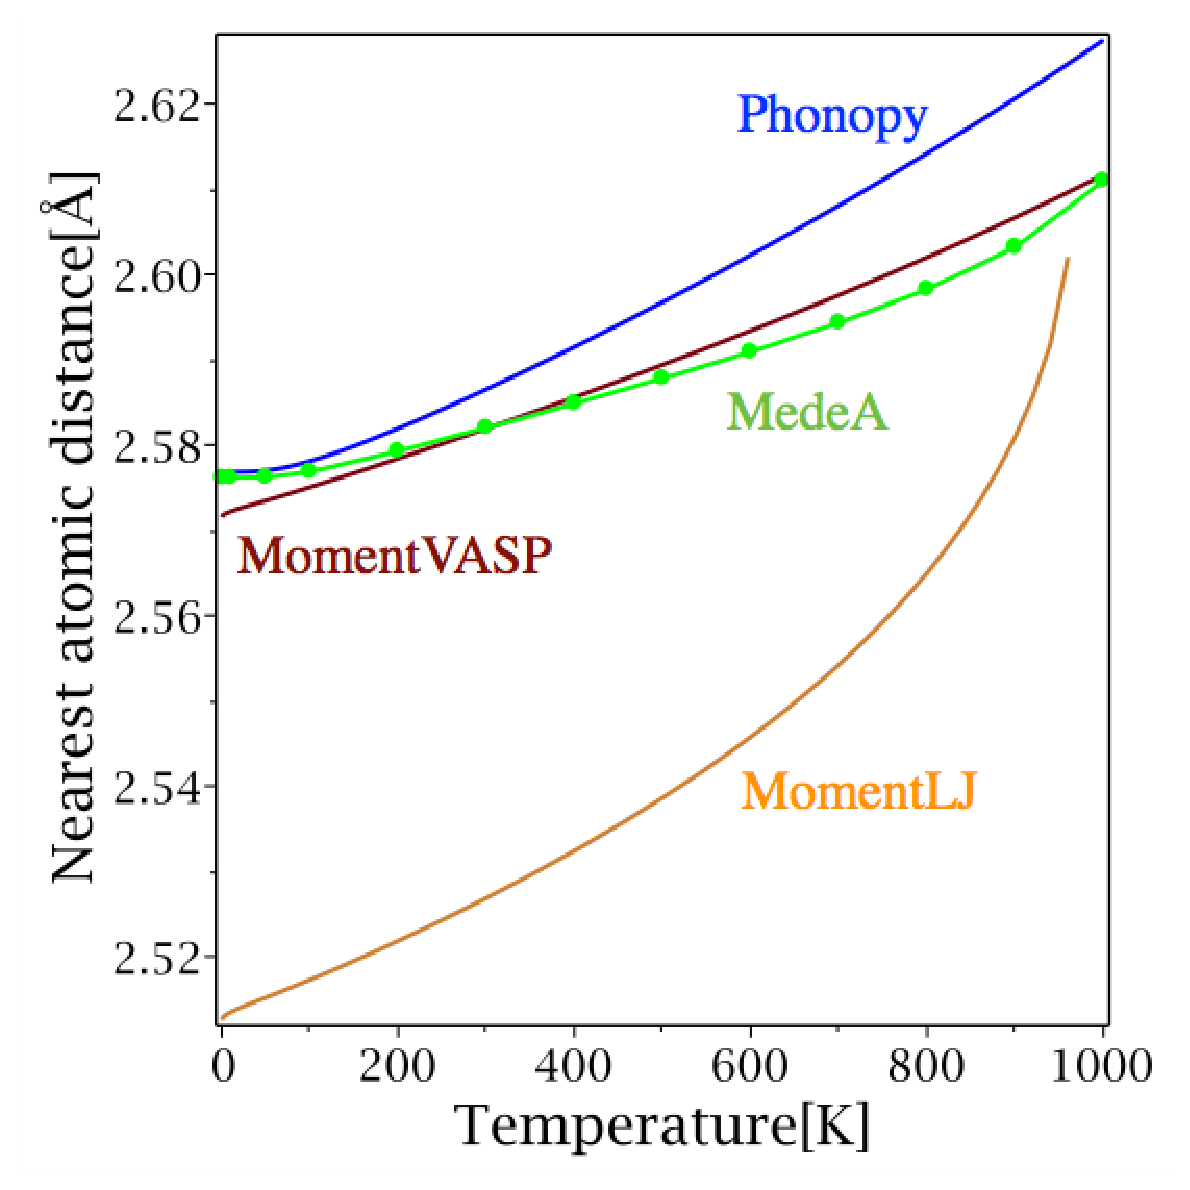
\includegraphics[width=4.7cm]{./image_result/Cu_lat_label.eps}
\subcaption{Cu.}
\end{center}
\end{minipage}
%\hspace{5mm}
\begin{minipage}{0.245\hsize}
\begin{center}
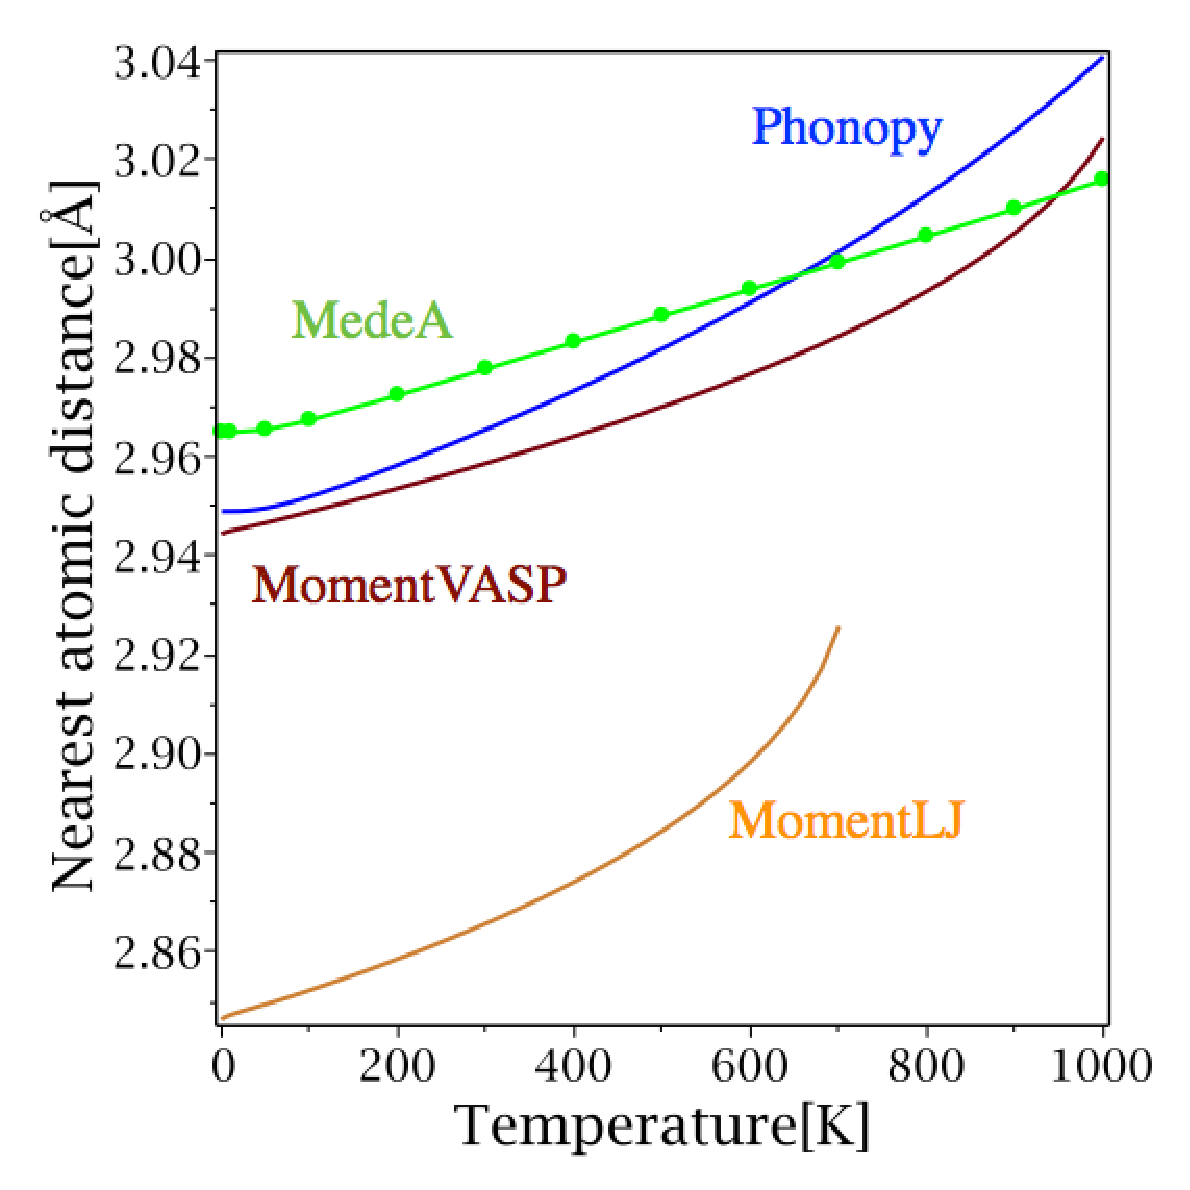
\includegraphics[width=4.7cm]{./image_result/Ag_lat_label.eps}
\subcaption{Ag.}
\end{center}
\end{minipage}
 \begin{minipage}{0.245\hsize}
\begin{center}
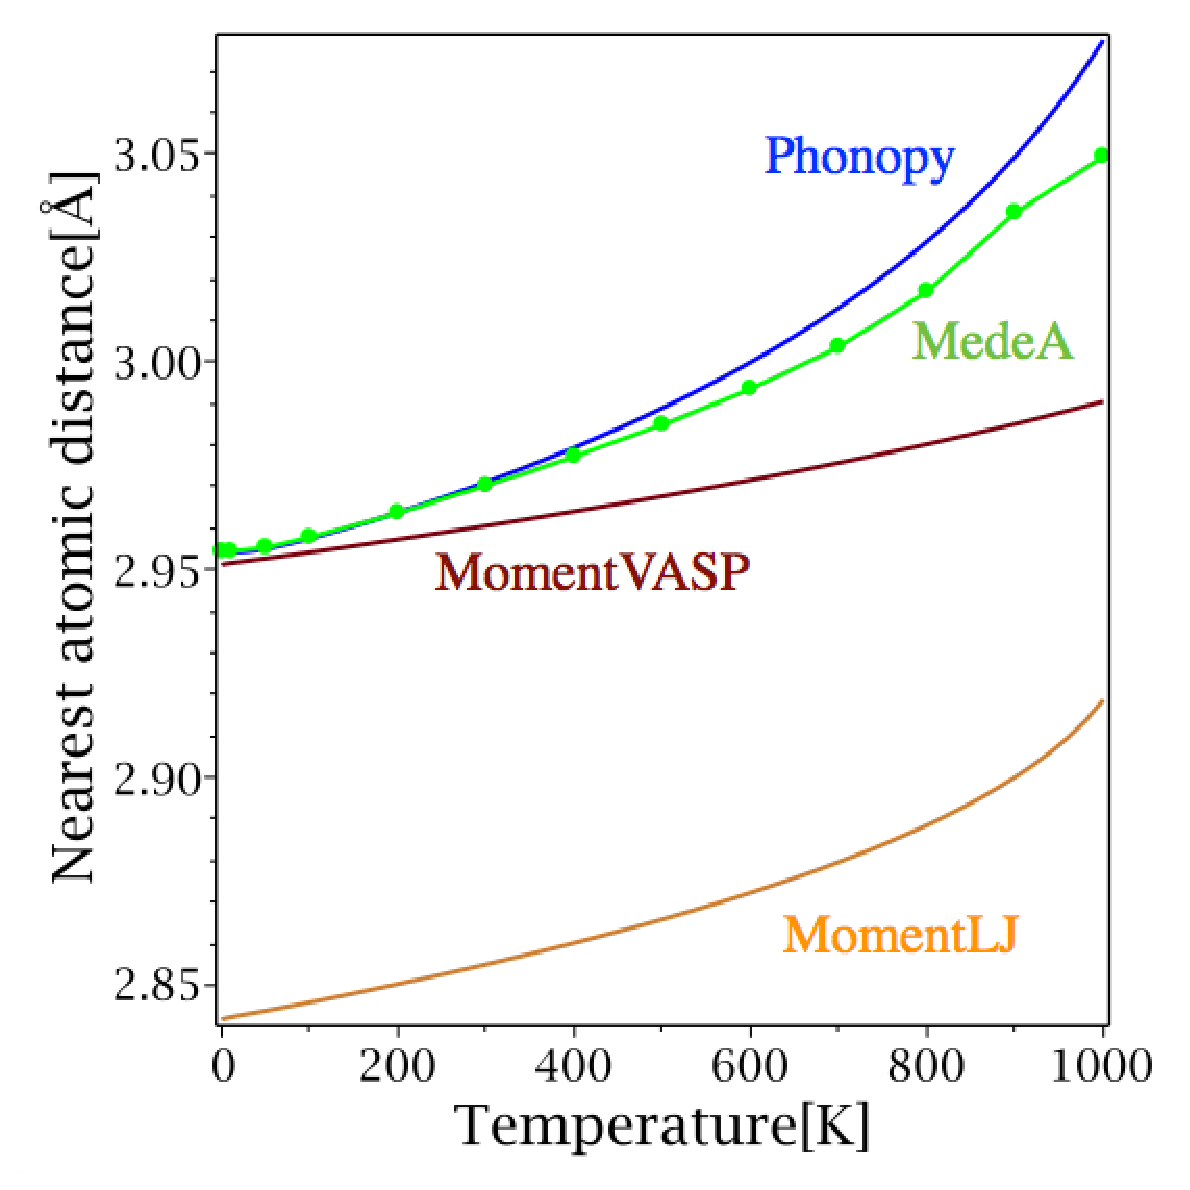
\includegraphics[width=4.7cm]{./image_result/Au_lat_label.eps}
\subcaption{Au.}
\end{center}
\end{minipage}
 \begin{minipage}{0.245\hsize}
\begin{center}
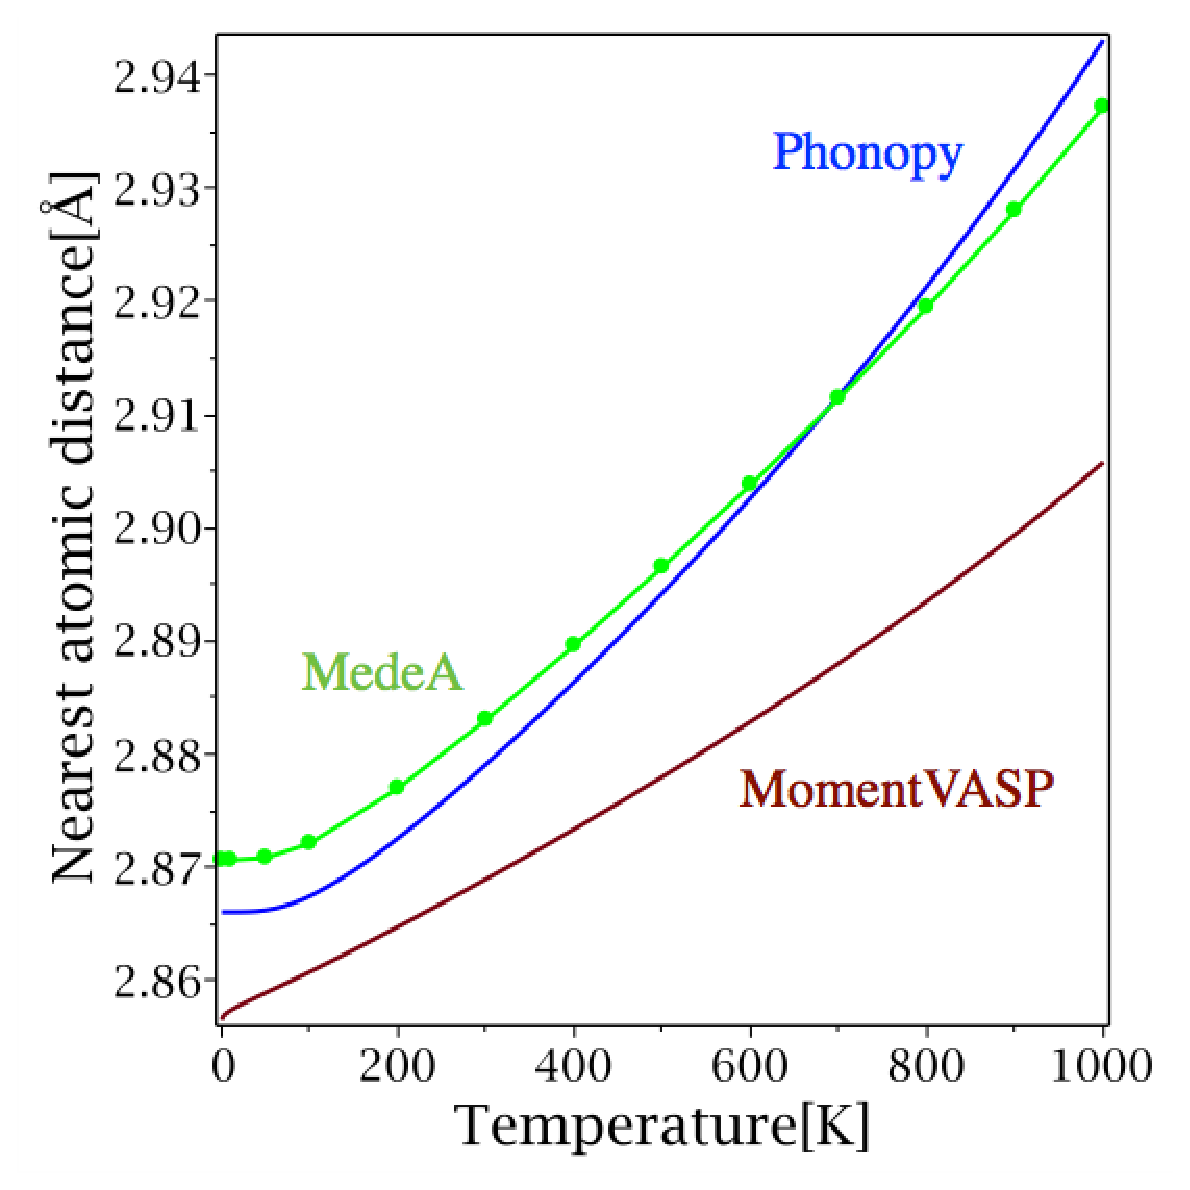
\includegraphics[width=4.7cm]{./image_result/Al_lat_label.eps}
\subcaption{Al.}
\end{center}
\end{minipage}
 \caption{最近接原子間距離の温度依存性.}
\end{figure*}

\begin{figure*}[htb]
\begin{minipage}{0.245\hsize}
\begin{center}
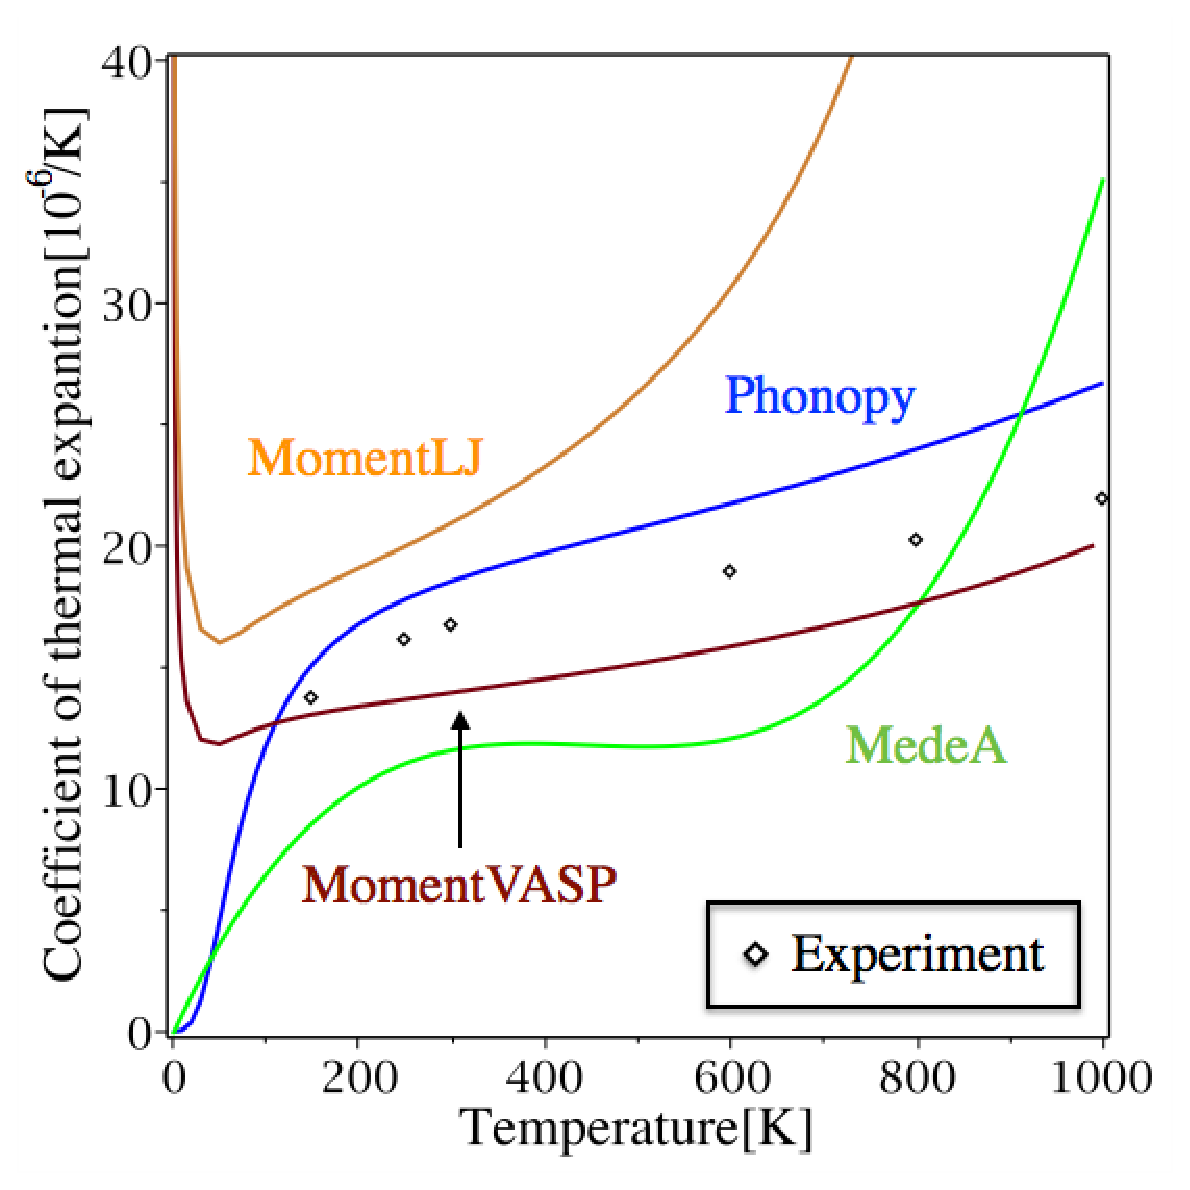
\includegraphics[width=4.7cm]{./image_result/Cu_TEcoeff_label.eps}
\subcaption{Cu.}
\end{center}
\end{minipage}
%\hspace{5mm}
\begin{minipage}{0.245\hsize}
\begin{center}
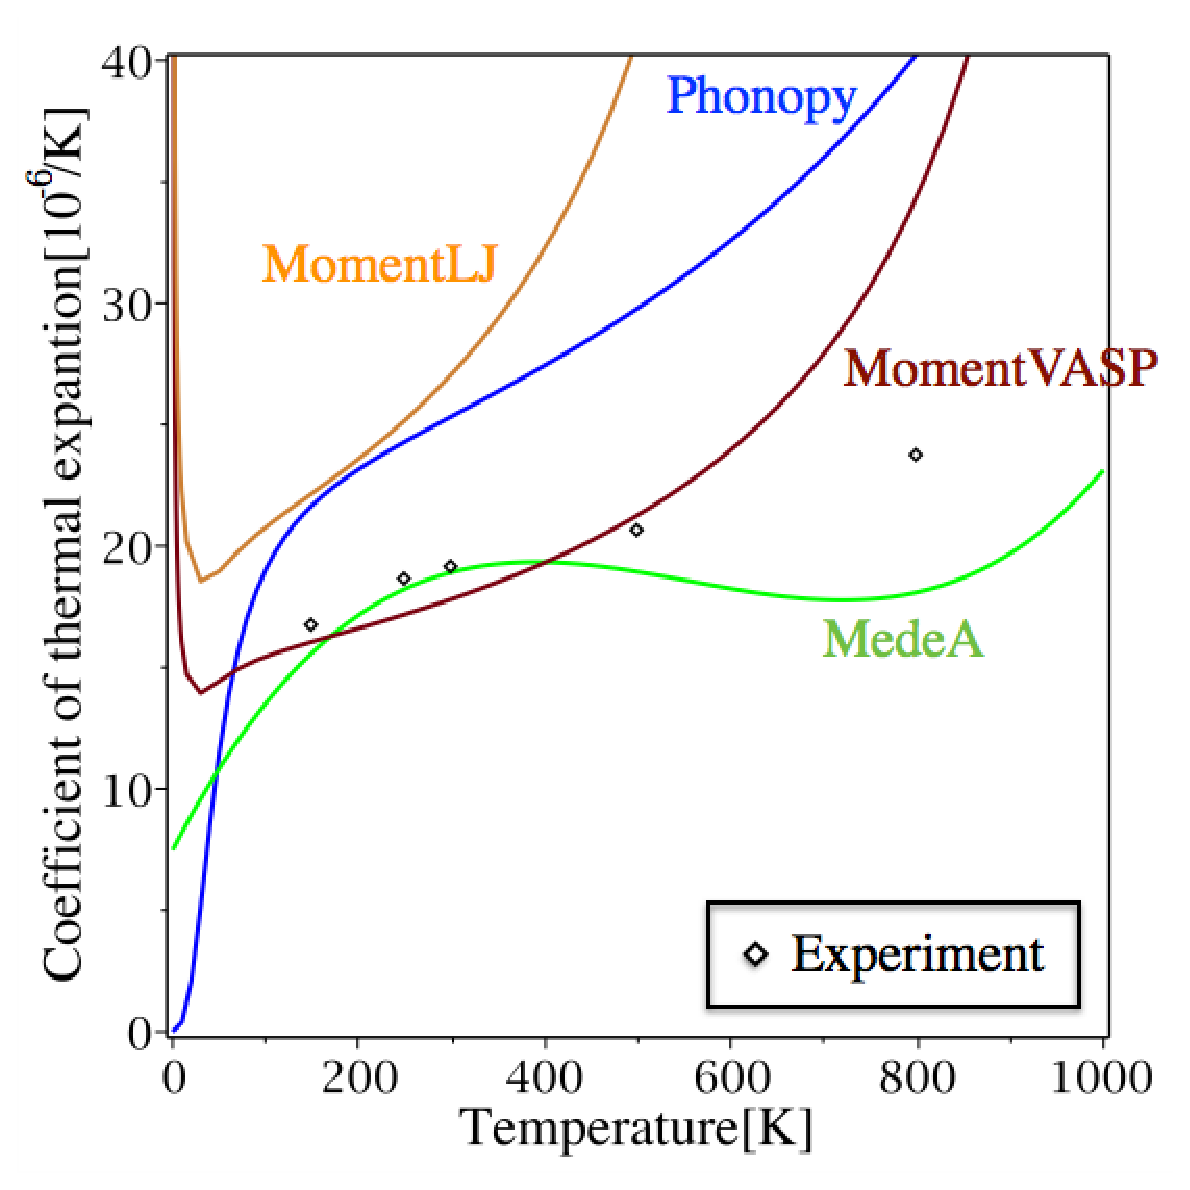
\includegraphics[width=4.7cm]{./image_result/Ag_TEcoeff_label.eps}
\subcaption{Ag.}
\end{center}
\end{minipage}
 \begin{minipage}{0.245\hsize}
\begin{center}
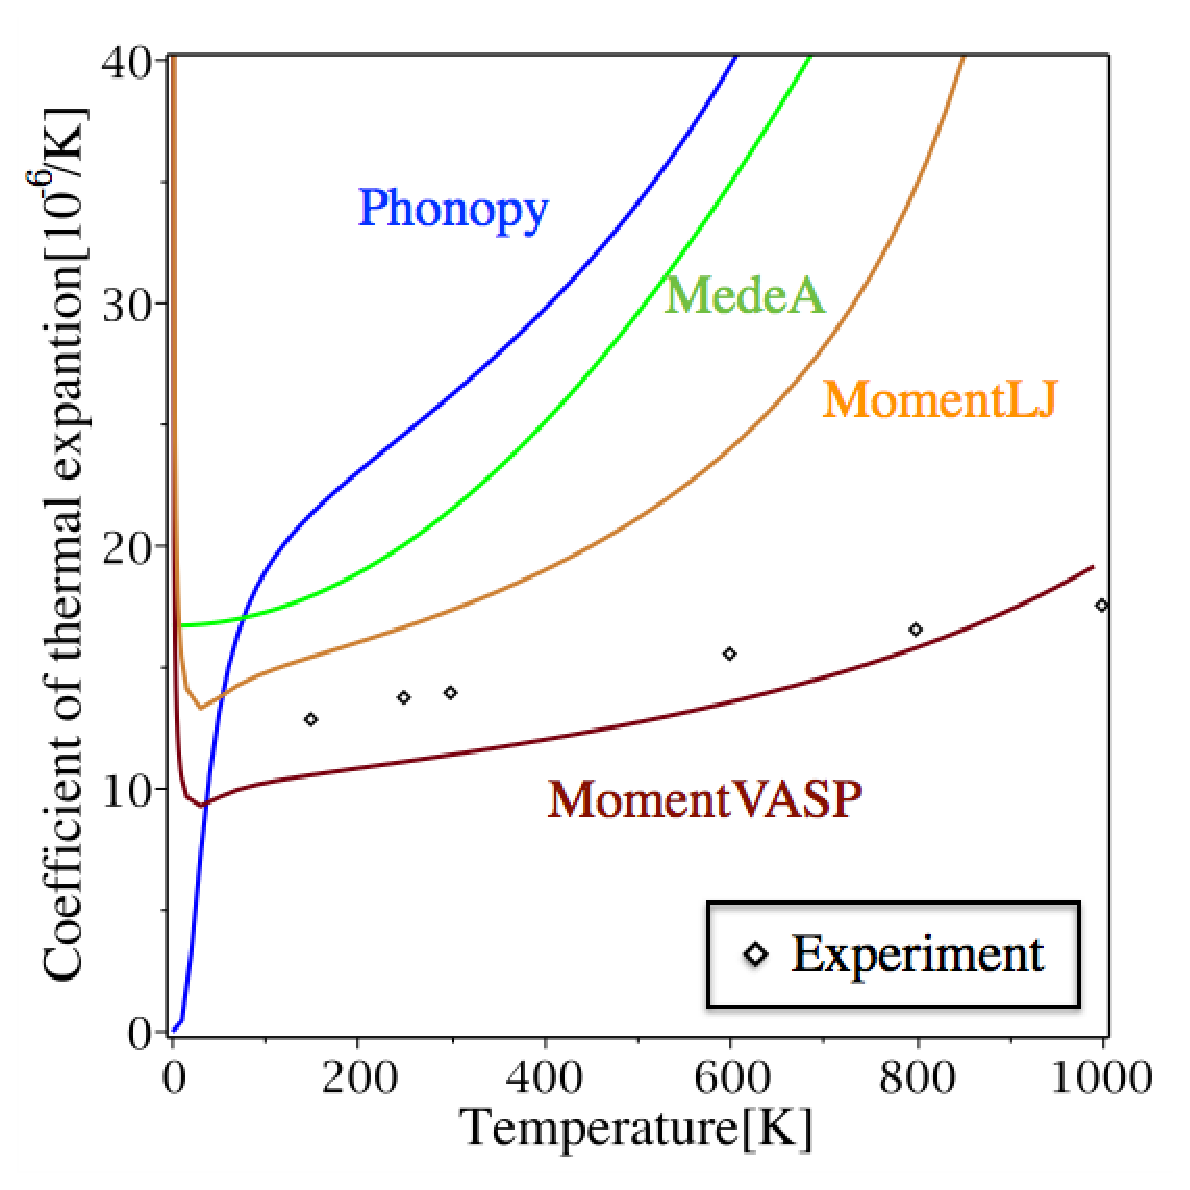
\includegraphics[width=4.7cm]{./image_result/Au_TEcoeff_label.eps}
\subcaption{Au.}
\end{center}
\end{minipage}
 \begin{minipage}{0.245\hsize}
\begin{center}
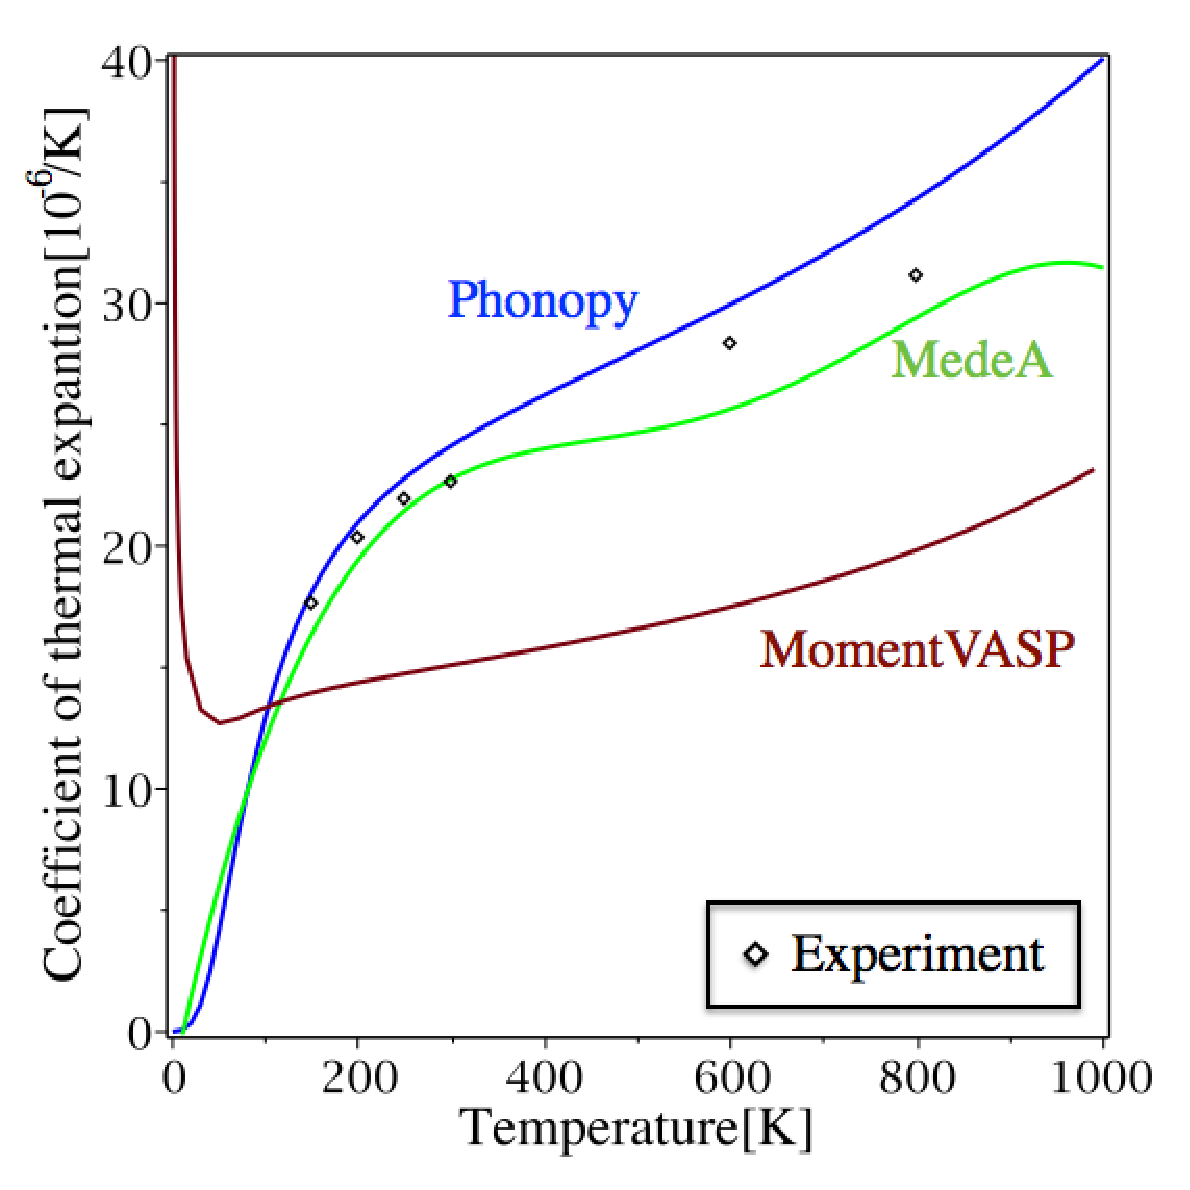
\includegraphics[width=4.7cm]{./image_result/Al_TEcoeff_label.eps}
\subcaption{Al.}
\end{center}
\end{minipage}
 \caption{線膨張係数の温度依存性.}
\end{figure*}

\begin{figure*}[htb]
\begin{minipage}{0.245\hsize}
\begin{center}
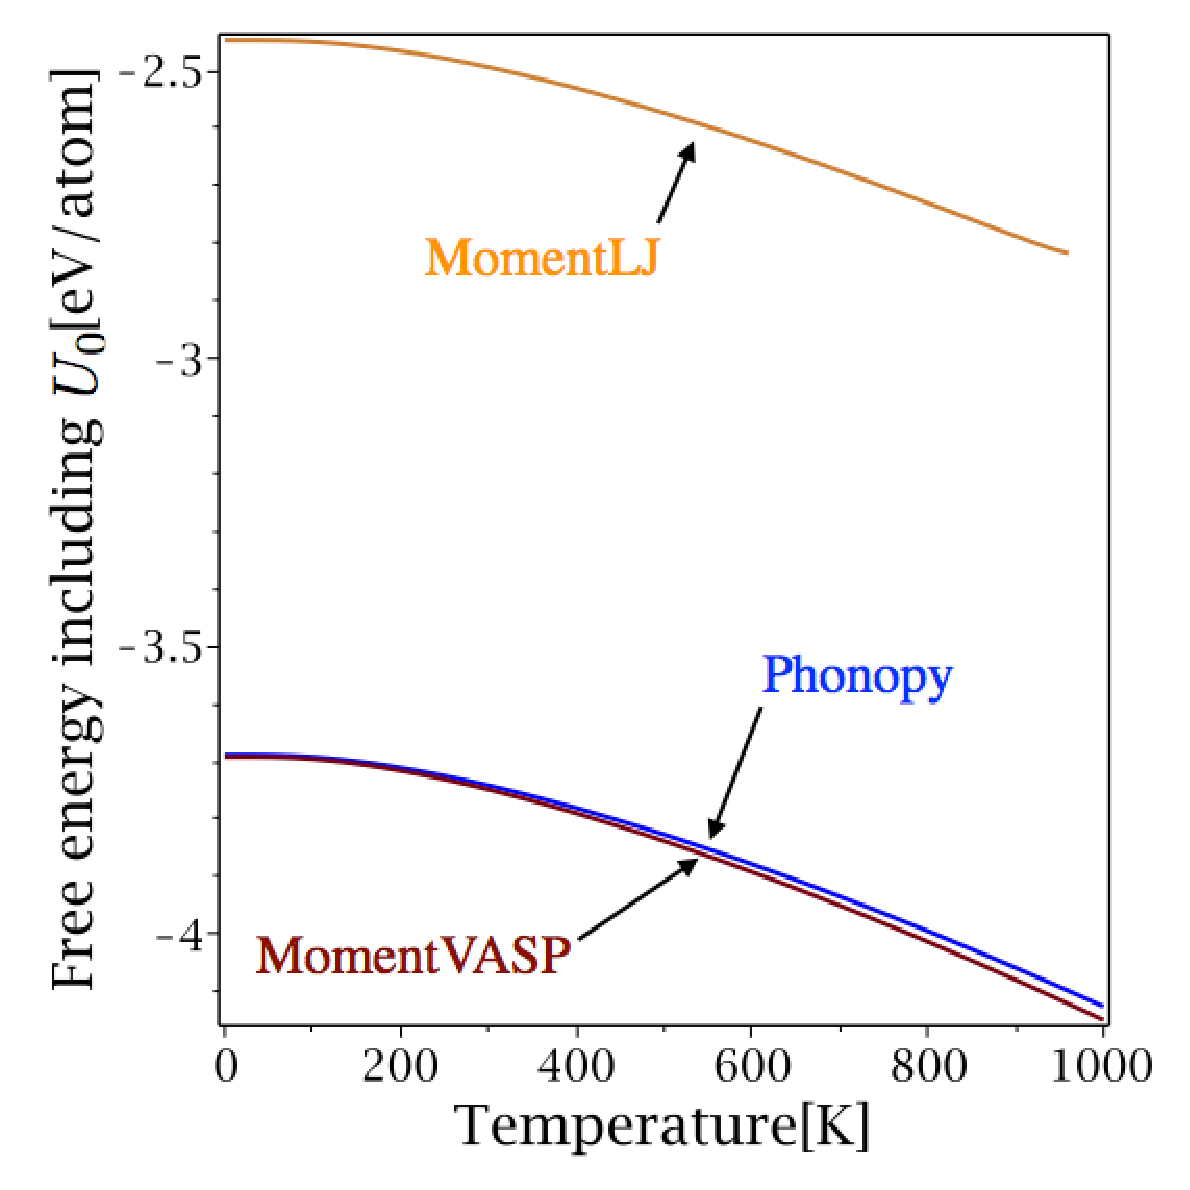
\includegraphics[width=4.7cm]{./image_result/Cu_free_u0_label.eps}
\subcaption{Cu.}
\end{center}
\end{minipage}
%\hspace{5mm}
\begin{minipage}{0.245\hsize}
\begin{center}
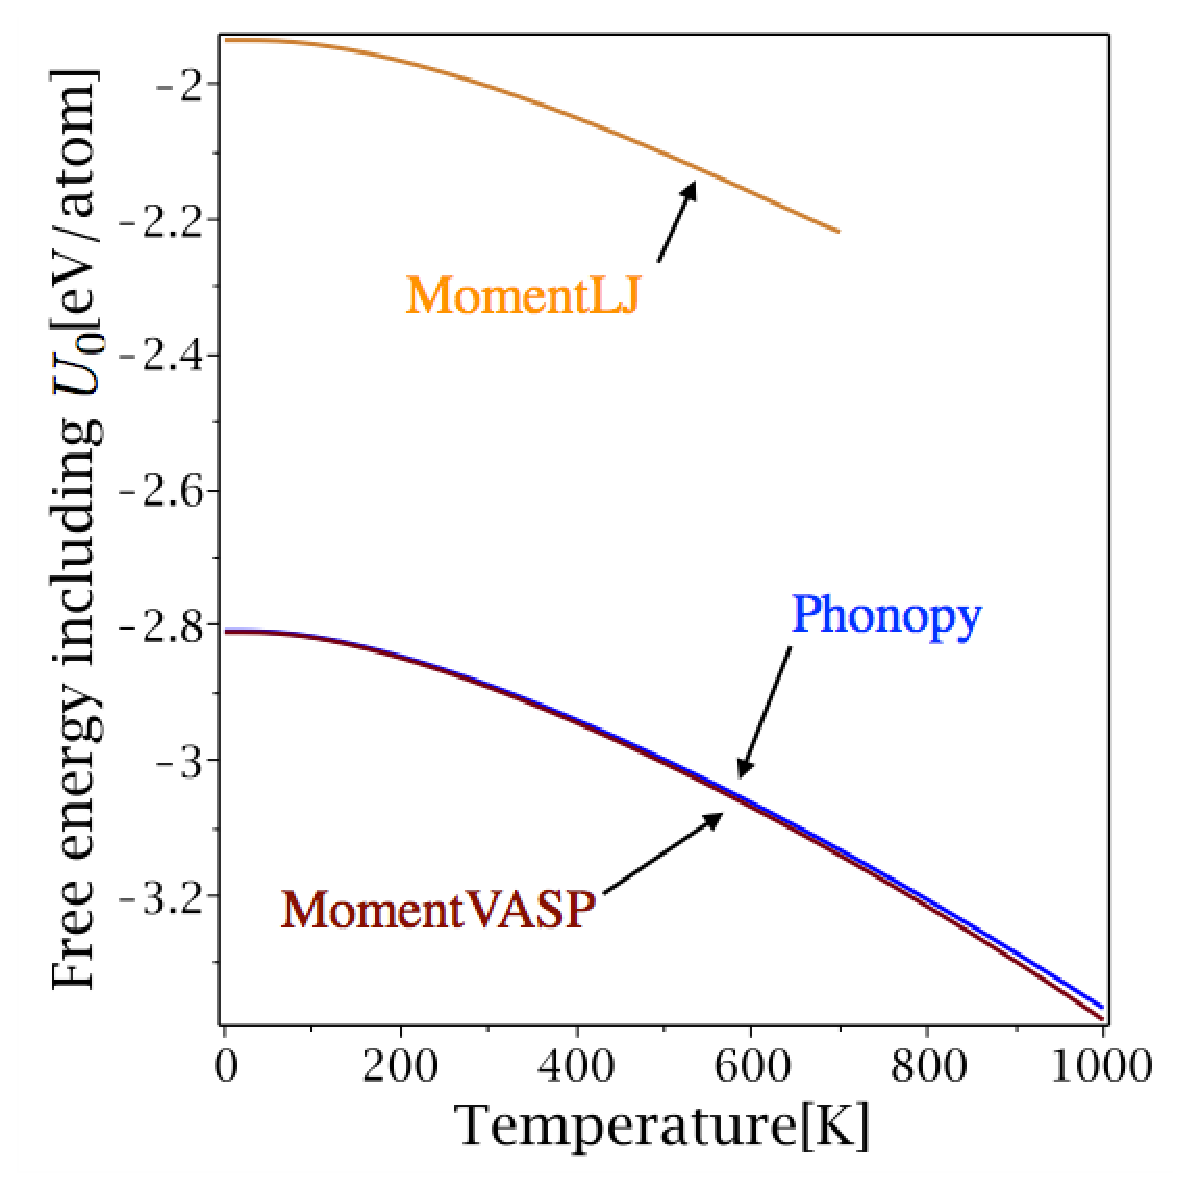
\includegraphics[width=4.7cm]{./image_result/Ag_free_u0_label.eps}
\subcaption{Ag.}
\end{center}
\end{minipage}
 \begin{minipage}{0.245\hsize}
\begin{center}
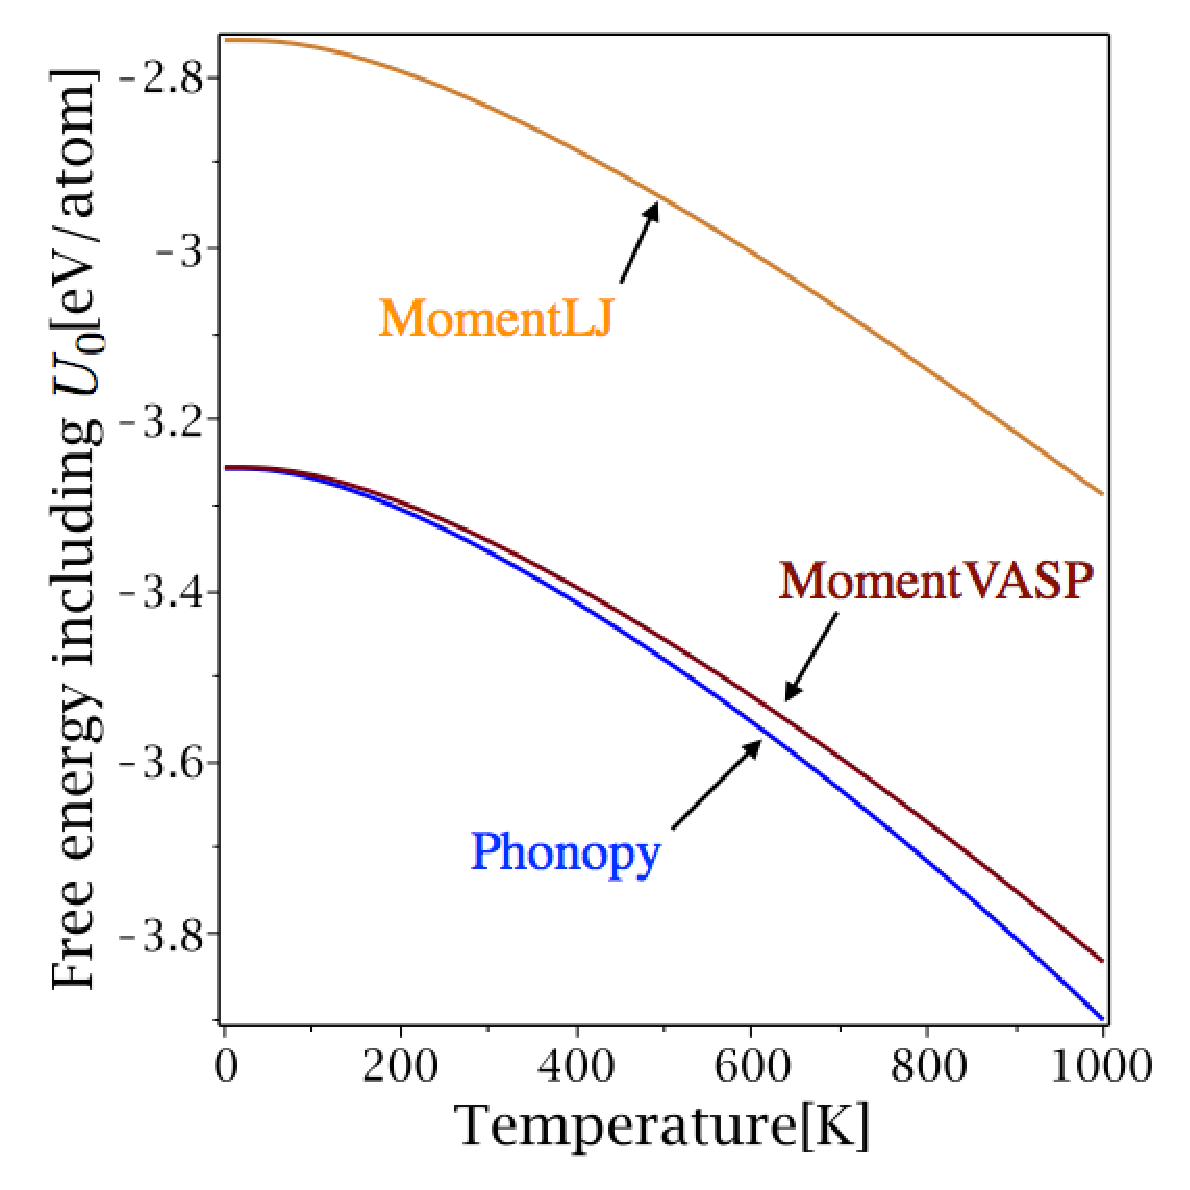
\includegraphics[width=4.7cm]{./image_result/Au_free_u0_label.eps}
\subcaption{Au.}
\end{center}
\end{minipage}
 \begin{minipage}{0.245\hsize}
\begin{center}
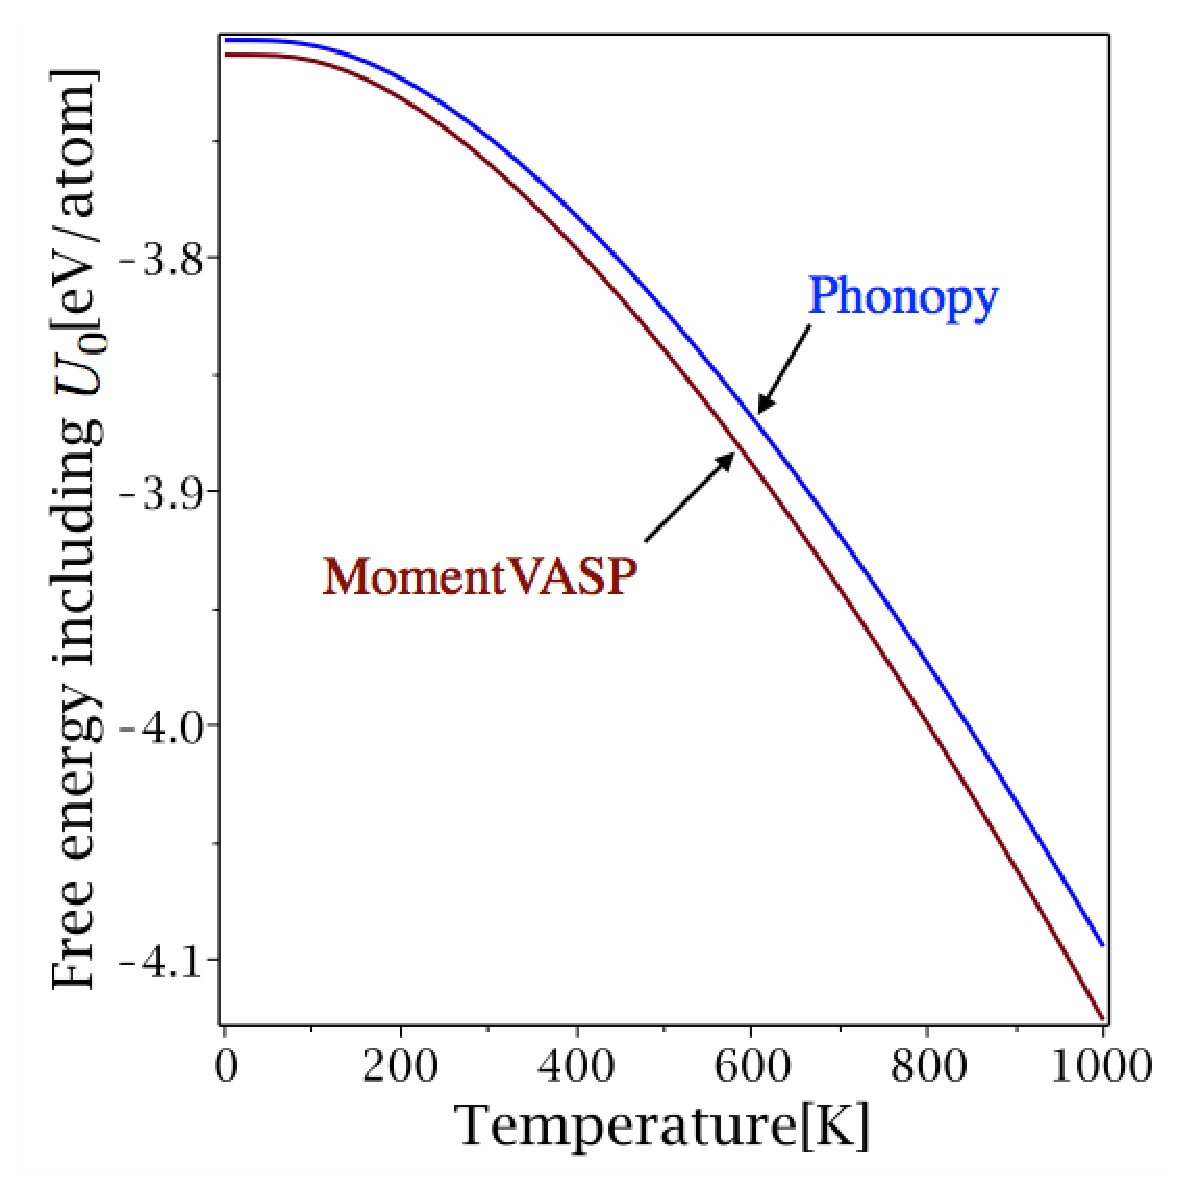
\includegraphics[width=4.7cm]{./image_result/Al_free_u0_label.eps}
\subcaption{Al.}
\end{center}
\end{minipage}	
 \caption{内部エネルギーと熱膨張を考慮した自由エネルギーの温度依存性.}
\end{figure*}

\subsection{自由エネルギー}
熱膨張が求まれば,その原子間距離における$k$, $\gamma$から自由エネルギーを計算できる.

\subsection{VASPの導入}
各元素のユニットセルに対して,VASPの構造最適化によって得られた格子定数を0.95
倍から1.10 倍まで0.01刻みで変化させエネルギーの計算を行い,得られた16点に対してフィッティングをおこなった.
fitting関数の$n$次までの基本形は次式となる.
\begin{eqnarray}
\label{eq:method2}
U(r)=a_0+a_1(r-x_0)+\cdots+a_n(r-x_0)^n
\end{eqnarray}
$x_0$は平衡原子間距離,$a_0$から$a_n$はフィッティングパラメータである.
今回は検討の末,4次微分した際に3次の項まで残る7次までのフィッティング関数を用いた.
フィッティングにより得られたポテンシャル関数はVASPの計算結果のため3次元を考慮している.
しかし,Moment法の熱膨張は線形結合を前提としているため,そのまま計算しても熱膨張を再現することができない.
そのため,今回はfcc構造が等方的であることからポテンシャル関数を3で割ることにより線形結合への対応を試みた.
これにより得られる関数の2次微分を$k$,4次微分を6で割ったものを$\gamma$とし計算をおこなった.

\section{結果}
図1にVASPを導入したMoment法,従来のMoment法,MedeA,Phonopyの熱膨張の結果を示す.
また,図2に熱膨張の温度微分である線膨張係数を示す.
VASPを導入したMoment法は,従来のMoment法と比べてMedeA, Phonopy, 実験値に近い値を出している.
Auの熱膨張はMedeA,PhonopyではPhononに負の値が混じり上手く再現できていないが,Phononとは違うアプローチで計算をするMoment法では実験に近い数値が出ている.
AlではMedeA, Phonopyは実験値をよく再現できているが,VASPを導入したMoment法は熱膨張が小さい結果となった.
図3に内部エネルギーと熱膨張を考慮した自由エネルギーの温度依存性を示す.
Cu, Agはよく一致しているが,Au, Alは熱膨張に差があることもあり異なるカーブを描いている.
\section{総括}
VASPを導入したMoment法は比較的良い結果が得られた.この手法は改善の余地があり今後の計算精度の向上が期待できる.今後の課題としては以下が挙げられる.

\begin{itemize}
\item 今回はfcc構造の等方性に注目し線形結合に対応するためにポテンシャルを3で割るという手法を試みたが,
もっと良い手法がないか検討を行う必要がある.
また,等方的ではないhcp構造ではどうするのか考える必要がある.
\item 今回の計算ではポテンシャルをフィッティングする際に7次の項まで利用したが,拾えていない成分が残っているかもしれない.そのため,フィッティング精度を高めてさらに高次の項まで取り込むなどの改善を期待する.
\end{itemize}

\bibliographystyle{jplain}
\renewcommand{\bibname}{参考文献}
\begin{thebibliography}{10}
\addcontentsline{toc}{chapter}{参考文献}
\bibitem{phonon}K. Parlinski, Z. Q. Li, and Y. Kawazoe, Phys. Rev. Let., {\bf 78} (1997), 4063-4066.
\bibitem{kiyohara}清原資之, 「Ti結晶多形におけるPhonon第一原理計算」, 関西学院大学 理工学部 卒業論文,2013. 
\bibitem{jindo}Vu Van Hung, and K. Masuda-Jindo, J. Phys. Soc. Jpn., {\bf 69} (2000), 2067.
%\bibitem{Hido}
%S.Hido et. al.
%\newblock A Linear-Time Graph Kernel.
%\newblock {In \textit{  Proceedings of the International Conference on Data Mining(ICDM)}}, pp. 179-188, (2009)
\end{thebibliography}
\end{document}